% NeurIPS 2026 workshop extended abstract.
% Requires neurips_2026.sty in this directory (official kit, revised January 2026).
% Build:  pdflatex context_fatigue.tex   (x2 for refs)
%
% Track option: `dblblindworkshop` anonymises the author block and adds line numbers.
% For a single-blind workshop swap it for `sglblindworkshop`; add `final` alongside
% either one for the camera-ready.

\documentclass{article}

\usepackage[dblblindworkshop]{neurips_2026}

\usepackage[utf8]{inputenc}
\usepackage[T1]{fontenc}
\usepackage{hyperref}
\usepackage{url}
\usepackage{booktabs}
\usepackage{amsmath}
\usepackage{amssymb}
\usepackage{microtype}
\usepackage{enumitem}
\usepackage{caption}
\usepackage{subcaption}
\usepackage{graphicx}

% compaction for a short extended abstract
\setlength{\textfloatsep}{7pt plus 2pt minus 2pt}
\setlength{\intextsep}{7pt plus 2pt minus 2pt}
\captionsetup{skip=3pt}
\captionsetup[sub]{skip=1pt}
\setlist[itemize]{nosep,leftmargin=1.4em,topsep=2pt}

\title{Context Rot Is Three Mechanisms:\\Only Displacement Acts Through Attention Mass}

% REQUIRED for the workshop track: the footnote on page 1 reads "Workshop: <this>."
\workshoptitle{WORKSHOP TITLE}

\author{%
  Ronen Raj Roy\\
  \texttt{ronex665@gmail.com}\\
}

\begin{document}

\maketitle

\begin{abstract}
Long conversations are said to wear language models down. The phenomenology is easy to
elicit---as context fills, output entropy collapses several-fold and the last token's attention
drifts off the system prompt and the current query onto recent text---but the causal claim behind
it has never been tested inside a single harness, because the standard setups confound
\emph{accumulation} (more context) with \emph{dilution} (the answer-bearing tokens becoming a
smaller, more distant fraction of it). We separate them. Accumulating \textbf{individually
localized} tasks, where the evidence for the current answer always sits at the current query, we
reproduce the full signature battery across four model families and find \textbf{no accuracy cost}
and no loss of instruction adherence. Holding items, model, fill and metric fixed and moving only
\emph{where the evidence lives}, the cost appears at once: displacing it costs $0.19$--$0.21$
accuracy, and in a joint fit distance carries the coefficient
($\beta{=}-0.0076$ $[-0.0117,-0.0035]$) while fill carries none. We then show this cost is
\textbf{causally mediated by attention mass}. Clamping the evidence's attention share at its
original position, with nothing moved, reproduces \textbf{114\%} of the displacement penalty
($+0.202$ $[+0.138,+0.267]$, landing indistinguishably on the displaced arm); a dose-response
sweep over the share recovers the same effect to within $0.004$ and shows the mass$\to$accuracy
curve is smooth and graded, with no threshold anywhere in it. The drain itself is positional in
\emph{tokens}, not turns. Holding distance and fill fixed and varying only how \emph{confusable}
the accumulated context is isolates a \emph{second and separate} cost: near-duplicate context is
worth $-0.085$ $[-0.140,-0.030]$ while leaving the evidence's \emph{total} attention mass
unchanged ($-0.0003$ $[-0.0009,+0.0004]$, where the measured dose-response predicts $2\%$ of the
observed effect). That null is layer-specific: measured across all $32$ layers the same contrast removes
$0.0022$ of evidence mass against displacement's $0.0455$, for accuracy costs of $0.085$ and
$0.188$---cheap in mass but not free, and the two drain profiles run in opposite directions across
depth. So displacement acts through attention mass and competition does not---and needle benchmarks
vary both at once, which is why they have not been told apart. A third mechanism costs
\emph{compliance} rather than accuracy: accumulated filler erodes an instructed output format
only when it demonstrates an answer shape applicable to the current probe---a drop-in shape
collapses compliance $0.875\to0.000$ by fill $0.15$, with accuracy unharmed, while off-domain
filler holds compliance ${\geq}0.88$ through fill $0.78$. That erosion is also not attention-mediated:
the instruction's per-token attention is flat-to-rising in every arm, masking the demonstrations
at generation time restores nothing, and the instruction stays perfectly linearly decodable
(AUC $1.000$) while behaviorally inert. Yet attention mass is a causal \emph{weight} in the
contest---clamping the instruction's share down collapses compliance ($0.99\to0.03$) where
nothing in context competes, clamping it up restores it against $42$ counter-exemplars, and
restating the policy restores it without surgery. Meanwhile the
signatures are in-context comfort: the entropy collapse vanishes on organic WildChat dialogue and
tracks conversation homogeneity, not length, and across OLMo-2's post-training chain it is a
baseline-confidence level shift installed mostly by SFT. Context rot, as measured, is not a decay
of competence with length: accumulation alone is free; what costs accuracy is the evidence being
displaced or contested, and what costs compliance is the model's own applicable precedent---and
only displacement is attention dilution.
\end{abstract}

\section{Introduction}

A recurring worry about long conversations is \emph{context rot}: as turns accumulate, the model
is said to degrade. The phenomenology is real. On a repeating multiple-choice task,
instruction-tuned models become dramatically more confident as context fills---next-token entropy
drops $3$--$4\times$ on Qwen-2.5-7B and Llama-3.1-8B, in both question orders---and the last
token's attention shifts systematically away from the system prompt and the current query toward
the most recent prior cases, with the distribution diffusing (at layer 24 of OLMo-2-Instruct:
system$\leftrightarrow$fill $-0.93$, recent$\leftrightarrow$fill $+0.89$,
current$\leftrightarrow$fill $-0.71$, entropy$\leftrightarrow$fill $+0.95$, all monotone in fill).
By every visual diagnostic this is a strong effect that grows with context.

The tempting reading is that the model is being worn down by length. But almost every
context-rot evaluation embeds the answer-bearing information inside \emph{one long task}---a long
document, a buried needle, a growing codebase. There, longer context mechanically \emph{dilutes}
the relevant tokens among irrelevant ones, so a measured degradation conflates the cost of
accumulation per se with the cost of the target being harder to attend to (``lost in the middle,''
\citealp{liu2023lost}). These cannot be told apart in that setup, and the distinction matters
practically: an agent transcript of finished, locally-scoped steps accumulates without diluting,
and the two accounts make opposite predictions about it.

In this paper we separate them inside one harness. We accumulate \textbf{individually localized}
tasks, so that context length and the dilution of the answer-bearing evidence become independent
knobs, and we intervene on each in turn. Accumulation alone costs nothing. Moving the evidence
$k$ turns back, at identical fill and byte-identical questions, costs $0.19$--$0.21$ accuracy
(Table~\ref{tab:distance}).

\begin{table}[t]
  \centering\small
  \caption{\textbf{Distance is the variable that matters} (OLMo-2-Instruct, $n{=}192$ per arm,
  chance $=0.200$, fill $0.688$ in every arm). Evidence attention share is measured at layer 24 on
  the same forwards. Case-resampled bootstrap 95\% CIs.}
  \label{tab:distance}
  \setlength{\tabcolsep}{4.5pt}
  \begin{tabular}{lccccc}
    \toprule
    arm & \texttt{local} & \texttt{back\_2} & \texttt{back\_5} & \texttt{back\_10} & \texttt{back\_20}\\
    \midrule
    accuracy & \textbf{0.464} & 0.359 & 0.292 & 0.250 & 0.276\\
    cost vs \texttt{local} & --- & $+0.104$ & $+0.172$ & $+0.214$ & $+0.188$\\
    95\% CI & --- & $[+.005,+.203]$ & $[+.073,+.266]$ & $[+.120,+.307]$ & $[+.094,+.281]$\\
    evidence share @L24 & 0.0408 & 0.0363 & 0.0320 & 0.0195 & 0.0124\\
    \bottomrule
  \end{tabular}
\end{table}

That cost is \emph{causally mediated by attention mass}. A clamp that sets a span's post-softmax
attention share lets us remove the evidence's mass while leaving it exactly where it is: doing so
reproduces $114\%$ of the displacement penalty, and a dose-response sweep over the share recovers
the same endpoint to within $0.004$ across two separately-run experiments.

A second cost is not mediated that way at all. Holding the evidence at the current query and
varying only how \emph{confusable} the accumulated context is, near-duplicate context costs a
further $0.085$ accuracy while the evidence's attention share does not move measurably---$2\%$ of
what the measured dose-response would require.

A third cost falls on \emph{compliance} rather than accuracy. Holding the evidence local and
accumulating filler behind a format instruction, the instructed output format survives off-domain
filler through fill $0.78$ but collapses from $0.875$ to $0.000$ by fill $0.15$---three
turns---of filler whose answers demonstrate a shape applicable to the probe, never to recover,
while accuracy on the same replies is untouched. The instruction's per-token attention is
flat-to-rising through the collapse, and the instruction remains perfectly decodable from the
residual stream while it has zero behavioral force; yet clamping its attention down collapses
compliance where nothing in context competes, and either clamping it up or restating the policy
fully restores compliance against forty-two counter-exemplars. Format erosion is a
\emph{precedent contest} in which attention mass is a causal weight but not the natural driver.

Taken together, context rot is three mechanisms with different signatures, and a
needle-in-a-haystack benchmark varies the first two at once, which is why they have not been
told apart.

Our contributions are as follows:

\begin{itemize}
  \item A harness that makes accumulation and dilution independent, by accumulating individually
        localized tasks whose evidence never moves. In it, accumulation alone costs no
        accuracy and no instruction adherence, with bounded nulls rather than point estimates.
  \item A causal mediation result for displacement: removing the evidence's attention mass with
        nothing moved reproduces $114\%$ of the displacement penalty, and the mass$\to$accuracy
        relationship is smooth and graded with no threshold in it.
  \item A dissociation establishing a \emph{second} mechanism: competition costs accuracy at
        constant attention mass, so ``attention dilution'' is the right account of displacement
        and the wrong account of competition.
  \item A \emph{third} mechanism at the compliance level: accumulated demonstrations erode an
        instructed format only when their shape is applicable, immediately and with accuracy
        unharmed. The erosion is not attention-mediated---but the instruction's attention mass
        is a causal weight in the underlying contest, and re-weighting or re-presenting the
        instruction each fully reverse it.
\end{itemize}

\section{Background}

\paragraph{Length as the suspected cause.}
Most evidence for context rot comes from setups where the answer-bearing information sits inside a
single long input. \citet{liu2023lost} showed that accuracy depends strongly on \emph{where} in the
context the relevant passage sits, dipping when it falls in the middle. \citet{levy2024same} held a
reasoning task fixed and padded the input with task-irrelevant text, finding degradation well
before the models' advertised context limits. \citet{hong2025contextrot} ran a broad sweep over 18
models and found that reliability falls with input length even on tasks as simple as retrieval and
replication, and that the fall is not uniform: it depends on how similar the needle is to the
question, and on whether distractors are present. \citet{laban2025lost} report a large multi-turn
degradation, but locate its cause in the model committing early to a wrong reading and failing to
recover---not in length as such.

\paragraph{Confusable context as a separate suspect.}
A second literature manipulates the \emph{content} of the surrounding context rather than its
length. \citet{shi2023distracted} insert an irrelevant sentence into grade-school math problems and
observe a sharp accuracy drop. In retrieval-augmented generation, \citet{cuconasu2024noise} find
that documents retrieved as relevant but not containing the answer act as distractors and degrade
accuracy.

\paragraph{Instructions versus demonstrations.}
Demonstrations can override a model's trained priors \citep{wei2023icldifferently} and, at
scale, its safety training \citep{anil2024manyshot}; hardcoded assistant turns exhibiting a
competing pattern flip instruction-following into pattern-following
\citep{camassa2026instructioninduction}, and instruction-derived and demonstration-derived task
representations are measurably distinct \citep{davidson2025taskrepresentation}. Closest to our
question, \citet{dongre2026attentioncloses} track attention from responses to the system prompt
declining over $50$ filler turns and show that hard-masking the instruction out of the window
collapses compliance. In each case the instruction's attention is measured alongside the
behavioral change or ablated outright, never \emph{set}; and the eroding demonstrations are
supplied by the experimenter rather than accumulated from the model's own benign replies.

\paragraph{What is not separated.}
In each of these setups the two candidate causes move together. Padding a prompt lengthens it
\emph{and} pushes the evidence further from the query; adding a distractor document does the same
while also supplying a competing answer. So a measured degradation cannot be assigned to
accumulation, to the evidence becoming distant, or to the surrounding text becoming confusable. A
mechanistic thread---\citet{liu2023lost}'s positional account, and attention-based explanations
generally---suggests attention as the channel, but attention is measured alongside these
manipulations rather than intervened on. This paper separates these factors inside one harness
and intervenes on attention directly.

\section{Preliminaries}
\label{sec:prelim}

\paragraph{Localized task streams.}
Our harness accumulates \textbf{individually localized tasks}: a stream of self-contained
$5$-option medical cases (DDXPlus, \citealp{tchango2022ddxplus}) or discrete factual questions
(MMLU, \citealp{hendrycks2021mmlu}). Each answer depends only on the \emph{current} question,
which always sits at the end of the context; prior turns are never required to answer it.
Accumulation therefore grows the context without ever diluting the information the current answer
needs. A reversed-question-order control removes difficulty-ordering confounds. Because a
$4$--$32$k window holds only tens of cases, we pool many independent accumulation sessions.

\paragraph{The dilution knob.}
The design's real value is that dilution becomes an \emph{independent knob}. Holding the item, the
model, the total fill and the metric fixed, we can move the evidence $k$ user turns back into the
accumulated transcript, with the question text byte-identical across arms and the same filler in
every arm. Distance and fill, welded together in a long-document setup, move independently here.
All causal experiments run on OLMo-2-7B-Instruct at layer 24, seed 42, with an overflow
guard that skips rather than truncates every item that would not fit whole---truncating a long
item near the window edge manufactures exactly the late-window cost under study.

\paragraph{The attention-mass clamp.}
To intervene on attention rather than position, we add a clamp that \emph{sets} a token span's
post-softmax attention share: a constant bias on the span's key columns scales its odds, and
softmax renormalizes, so nothing in the attention forward is reimplemented and a scale of $1.0$
is bit-identical to the unhooked model. The clamp is uniform across heads.

\paragraph{Analysis.}
Per-condition $n$ is bounded by the context window, so every clamp experiment is paired over
shared items and analysed with a paired bootstrap resampling \emph{cases} (10,000 draws), never
heads or turns.

\section{Results}

\subsection{Accumulation}
\label{sec:accumulation}

Per-case accuracy does not fall as context fills; it is worst at the cold start and warms up
($\mathrm{corr}(\text{correct},\text{fill})=+0.11$ Instruct, $+0.07$ DPO). The obvious objection is
that a homogeneous repeating task lets in-context learning mask a hidden decay, so we remove that
crutch: in a \emph{random-subject} stream each question is drawn uniformly from all 56 MMLU
subjects, so prior context carries no predictive information about the next question---only the
answer \emph{format} is learnable. Accuracy is still flat (random: $\mathrm{corr}=-0.02$
$[-0.10,+0.05]$, $n{=}699$; coherent single-subject: $\mathrm{corr}=+0.01$, $n{=}1001$). These
nulls are \emph{bounded}: the 95\% interval on upper-minus-lower-half accuracy excludes declines
beyond $4.1$ points (coherent) and $9.4$ (random). Checkable instruction adherence---a canary
system instruction to begin every reply with a marker and end with a tag---stays at ceiling
throughout ($\mathrm{corr}(\text{violation},\text{fill})=0$), an honest null that bounds rather
than proves, since the canaries were easy; \S\ref{sec:precedent} shows what it does and does
not mean.

\begin{figure}[t]
  \centering
  \begin{subfigure}{0.33\textwidth}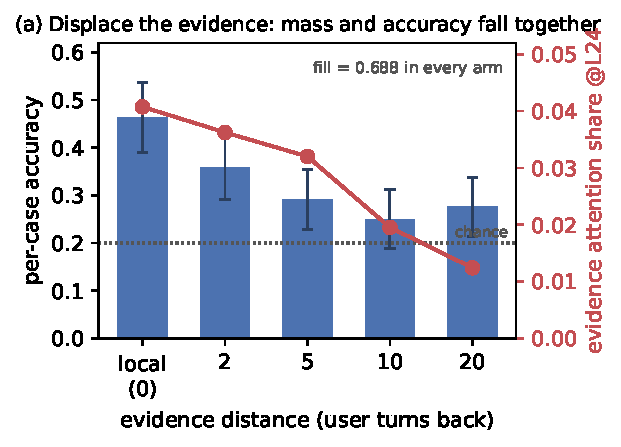
\includegraphics[width=\linewidth]{figures/distance_ladder.pdf}\end{subfigure}
  \hfill
  \begin{subfigure}{0.33\textwidth}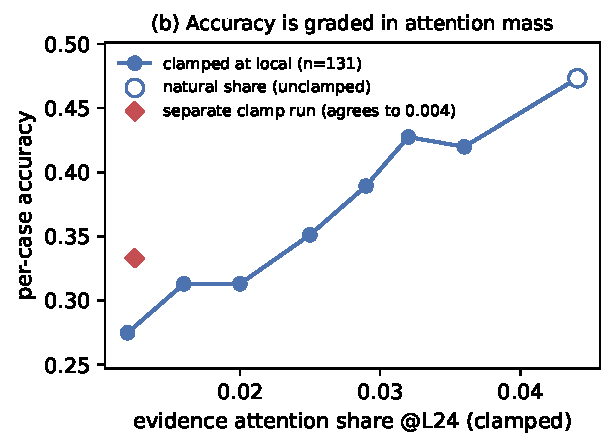
\includegraphics[width=\linewidth]{figures/mass_dose.pdf}\end{subfigure}
  \hfill
  \begin{subfigure}{0.33\textwidth}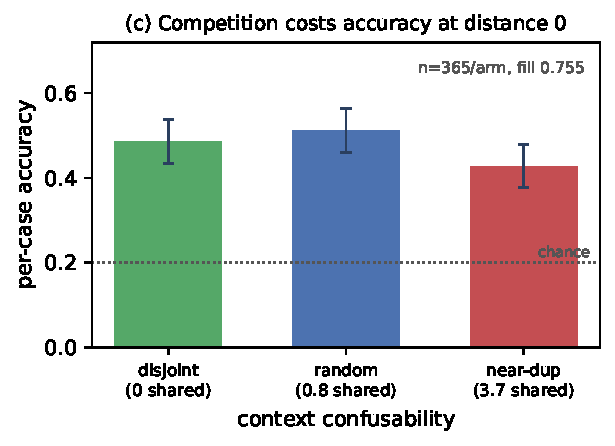
\includegraphics[width=\linewidth]{figures/competition.pdf}\end{subfigure}
  \caption{\textbf{Dilution costs accuracy; accumulation does not.}
  (a) Moving the evidence $k$ user turns back, at identical fill and byte-identical questions,
  drains its attention mass and costs accuracy together.
  (b) Setting that mass directly, with the evidence left in place, reproduces the penalty and
  traces a smooth graded dose-response---no threshold. The diamond is an independently-run clamp
  experiment measuring the same endpoint cut; the two agree to $0.004$.
  (c) At distance $0$ and fixed fill, near-duplicate accumulated context costs a further
  $0.085$. Bootstrap CIs resample cases throughout.}
  \label{fig:dilution}
\end{figure}

\subsection{Displacement}
\label{sec:displacement}

We now vary only \emph{where the answer-bearing evidence lives}. Each DDXPlus probe's vignette is
placed $k$ user turns before its question; mean fill is $0.688$ in every arm, the question text is
byte-identical, and the overflow guard skipped $0$ of $192$ probes. Every gap's CI excludes zero
(Table~\ref{tab:distance}, Fig.~\ref{fig:dilution}a). In a joint fit of accuracy on fill and
distance, \textbf{distance carries the coefficient} ($\beta=-0.00761$ $[-0.01173,-0.00346]$,
significant) and \textbf{fill carries none} ($\beta=-0.00725$ $[-0.21006,+0.18658]$). Within the
\texttt{local} arm---the one that reproduces the paper's original design---accuracy is flat with
fill ($\beta=-0.294$ $[-0.767,+0.184]$). The effect survives restriction to parsed responses and
is then fully monotone ($0.524\to0.413\to0.397\to0.343\to0.338$). One honest qualification: the
decline saturates by $k{\approx}10$ rather than deepening to $k{=}20$, and those two arms are not
distinguishable from each other. So the same model, on the same items at the same fill, degrades
when the evidence is displaced and does not degrade when it is not. The localized null is not a
ceiling artifact: these items \emph{can} show degradation, and do, as soon as dilution is
reintroduced.

Distance and attention drain move together by construction, so Table~\ref{tab:distance} is
consistent with dilution but does not establish it---a purely positional account predicts the same
table. Four interventions separate them.

\paragraph{Observational correlations.}
Evidence share falls $0.0408\to0.0124$ across the ladder ($r=-0.83$ with distance) while the
\emph{question}'s share stays flat, confirming only the evidence moved. A trap worth recording:
\emph{within} an arm, higher evidence share predicts \emph{lower} accuracy
($\beta=-11.2$ $[-20.0,-2.6]$, stronger controlling for vignette length). Attention there tracks
item difficulty---the model looks harder at confusing vignettes---and has the \emph{opposite sign}
to the causal effect below. Anyone reading share-against-accuracy correlations off this data
without intervening will conclude the reverse of the truth.

\paragraph{Mass removal.}
Keeping the evidence at \texttt{local} and clamping its share down to the \emph{same item's own}
\texttt{back\_20} share costs $+0.202$ $[+0.138,+0.267]$ (paired $n{=}174$) and lands at $0.333$
against \texttt{back\_20}'s $0.365$---a difference of $-0.025$ $[-0.083,+0.035]$, indistinguishable.
\textbf{Mass removal alone reproduces 114\% of the displacement penalty, with nothing moved.}

\paragraph{Dose-response.}
Sweeping the evidence's share at fixed position over seven levels (common subset $n{=}131$ present
at every level) gives a monotone decline from $0.473$ at the natural share ($0.0441$) to $0.275$ at
$0.012$ (Fig.~\ref{fig:dilution}b). Six of the seven levels differ significantly from the natural
share---including a cut of less than a fifth of the mass---and no step is a threshold: the largest
adjacent step is $0.053$ and the decline is smooth throughout. The endpoint contrast,
$+0.198$ $[+0.115,+0.282]$, matches the independently-run clamp experiment's
$+0.202$ $[+0.138,+0.267]$ for the same share change---agreement to $0.004$ across two separate
runs, which is the strongest internal consistency check in the program. An earlier draft of this
work read a \emph{threshold} into two flat contrasts; the sweep refutes it. The relationship is
\emph{graded}: a measured slope, not a cliff.

\paragraph{Mass restoration.}
The converse is only partial: clamping the displaced evidence's share back \emph{up} to its
\texttt{local} level---share-matched across all $32$ layers, not indexed to one---recovers a
real but small $0.28$ $[0.07,0.61]$ of the penalty ($+0.047$ $[+0.010,+0.083]$ of
$+0.167$ $[+0.099,+0.240]$), leaving most of it in place. Our
uniform clamp can strip mass faithfully but cannot reconstruct \emph{which} heads should carry the
restored mass. Full sufficiency with partial necessity is the signature of an instrument that is
faithful in one direction and crude in the other, and we report it as one rather than as a second
mechanism. A pattern-matched, per-head clamp is the test that would settle it.

\paragraph{Tokens versus turns.}
A partial $2{\times}2$ in (gap turns) $\times$ (filler length), total context equalized by padding,
dissociates them: two arms matched on \emph{tokens} have effectively identical evidence share
($0.0104$ vs $0.0108$) despite a $4\times$ difference in turn count, while at matched turns share
falls $0.0288\to0.0104$ as the gap grows $446\to1684$ tokens---a $64\%$ cut in the evidence's
attention that costs at most $9.4$ accuracy points ($+0.026$ $[-0.042,+0.094]$). Share regresses significantly on gap
tokens and not on gap turns. Attention drain is a function of token distance, as RoPE decay
predicts; conversation structure is not what drains it.

\paragraph{The current query.}
Accumulation drives the \emph{current query}'s share from ${\approx}0.35$ down to ${\approx}0.15$,
and it is natural to ask whether that stops short of a floor. It does not. Clamping the query span
on cold-start contexts, accuracy is flat from the natural share ($0.258$, accuracy $0.545$) down
through $0.20$ ($0.509$), then costs $16.4$ points at $0.15$ ($+0.164$ $[+0.036,+0.291]$)---which
is exactly the share accumulation reaches. Accumulation does not stop far short of the shoulder;
it stops \emph{at} it. (Levels below $0.15$ require $-4.7$ to $-6.1$ nats, near-ablation rather
than points on a dose-response---the model answers ``A'' $110/110$---and are excluded from
interpretation.) That accuracy nonetheless stays flat under accumulation, while the same share
reached by clamping costs points, is itself evidence that in-context learning is actively holding
accuracy up.

\subsection{Competition}
\label{sec:competition}

Burying a needle varies two things at once: the evidence becomes distant \emph{and} it becomes
surrounded by plausible alternatives. So far we have isolated distance. We isolate the other half by
holding the evidence at the current query and fill fixed, and varying only how \emph{confusable}
the accumulated context is. Every arm accumulates eight prior DDXPlus cases, each answered in the
transcript with its gold letter, so format and in-context-learning affordance are constant; the
arms differ only in how much the accumulated cases' differentials overlap the current probe's
(\texttt{disjoint} $0$ shared options, \texttt{random} $0.80$, \texttt{near\_dup} $3.75$ of $5$,
always with a \emph{different} gold, so the context never displays the probe's answer as a correct
one). Paired over $n{=}365$ probes, accuracy is \texttt{random} $0.512$, \texttt{disjoint} $0.485$,
\texttt{near\_dup} $\mathbf{0.427}$.

Near-duplicate context costs $-0.085$ $[-0.140,-0.030]$ against the natural stream and $-0.058$
$[-0.112,-0.006]$ against disjoint context; in a joint fit within this experiment, \textbf{option
overlap carries the coefficient} ($\beta=-0.021$ $[-0.039,-0.003]$) and \textbf{fill carries none}
($\beta=-0.284$ $[-0.640,+0.075]$)---the same shape as the distance result, on a different
variable. Two controls matter: the low-competition arms must land on \S\ref{sec:displacement}'s \texttt{local} accuracy
of $0.464$, and both do ($+0.049$ $[-0.037,+0.134]$ and $+0.021$ $[-0.065,+0.107]$); and context
length does not order the arms, since \texttt{disjoint} is the \emph{longest} and mid-accuracy
while \texttt{near\_dup} is the shortest, so length biases against the result. Restricted to
parsed responses only, \texttt{random} $-$ \texttt{near\_dup} $=+0.082$ $[+0.025,+0.138]$ survives.
The effect is \emph{not} monotone in confusability: \texttt{random} sits above \texttt{disjoint},
not below it, though not significantly ($+0.027$ $[-0.019,+0.074]$). Mild topical overlap
plausibly supplies useful priming over the option space while near-duplication supplies
competitors that actively mislead; only the second is large enough to measure here. We therefore
claim that near-duplicate context is costly, \emph{not} that cost rises with overlap---one
significant step, not a gradient.

\paragraph{Attention mass under competition.}
Repeating the sweep with attention capture instead of generation (same probes, same seeds), and
measuring every one of the model's $32$ layers rather than a reference layer, separates the two
mechanisms on mass. Averaged over all layers, displacement removes $0.0455$ of the evidence's
attention share and competition removes $0.0022$, while costing $0.188$ and $0.085$ accuracy
respectively. Competition is therefore far cheaper in mass per point of accuracy than
displacement, which is the dissociation---but it is \emph{not} mass-neutral, and the layer chosen
decides how it looks. At layer 24 the headline contrast moves the evidence's share by $-0.00027$
$[-0.00088,+0.00035]$, indistinguishable from zero; at layer 17 it moves it by $-0.0186$, and at
layers 16 and 18 by $-0.0110$ and $-0.0093$. The two drain profiles are moreover \emph{negatively}
correlated across layers ($r{=}-0.32$): displacement bites hardest at layers 0--3 and 16,
competition at 17--18. That the same accuracy contrast has opposite attention signatures in
different layers is evidence for two mechanisms which no single-layer measurement could supply.
An earlier version of this work reported that reproducing competition's cost through mass would
need a share change $50\times$ larger; that figure was read off layer 24 alone and does not hold
across the model.

\paragraph{Per head.}
Attention share is a mean over a layer's $32$ heads, and a mean can hold still while heads cancel,
so we also measured all $1{,}024$ heads. Under displacement at layer 24, \textbf{every head loses
evidence mass} from \texttt{local} to \texttt{back\_20}, each significant at Bonferroni, so nothing
is hidden by averaging. The loss is close to uniform in proportion---mean fractional drain $0.689$
(sd $0.147$), uncorrelated with how much mass a head held ($r{=}0.08$)---and a single uniform
odds-scale reproduces $58\%$ of the per-head pattern, which weakens (without eliminating) the
reading of \S\ref{sec:displacement}'s partial necessity as pure instrument limitation. Under
competition at the same layer the net is $0.0003$ while heads move $0.0026$ against a paired
sign-flip null of $0.0004$ ($p\leq0.0005$, 2{,}000 permutations), with $19$ of $32$ heads
individually significant: a small reallocation, about $6\%$ of the evidence's local share, rather
than inaction. Finally, heads that concentrate on the evidence do exist---$255$ of $1{,}024$
attend it more than its token share warrants, up to $0.626$ for one head on a span that is $0.102$
of the context---but none of them are at layer 24, whose mean evidence share ($0.0408$) is among
the lowest in the model. Conclusions about head specialisation drawn from a single layer do not
generalise, and we draw none.

\subsection{Precedent}
\label{sec:precedent}

The costs so far are to accuracy. A third mechanism costs \emph{compliance}: not whether the
model can still solve the task, but whether it answers in the instructed form. The system prompt
carries a clinical answer template (\texttt{ANSWER:} letter, then \texttt{SUPPORTING:} with at
least two vignette findings), the context accumulates the model's own replies to interleaved
filler, and every probe reply is graded separately for compliance and accuracy ($n{=}40$ probes
per depth, one accumulation snapshotted at every depth, so depth is the only mover).

\paragraph{The instruction's attention is causally necessary---and demonstration masks it.}
Accumulation drives the system span's share down $8\times$ within eight turns
($0.166\to0.021$). Clamping it from $0.165$ to $0.050$---a level accumulation passes on its own
between two and four turns, at $-2.6$ nats, well clear of the near-ablation regime excluded in
\S\ref{sec:displacement}---in a context containing no assistant turn collapses compliance from
$0.99$ to $0.03$ (a suffix canary flips on $120$ of $120$ items) while accuracy moves
$0.525\to0.467$ ($[-0.017,+0.133]$) at parse rate $0.967$: compliance is destroyed and
competence is not. But one \emph{compliant} example in context pins compliance at ceiling at
every clamp level, and one bare-letter example pins it at floor even unclamped---replies
byte-copy the previous assistant turn's format, with zero length variance across $720$
generations per arm. The instruction governs behaviour only when the transcript is silent,
which re-reads \S\ref{sec:accumulation}'s adherence null: that null accumulates
\emph{compliant} history, so it shows compliance survives compliant precedent, not accumulation.

\paragraph{Erosion tracks applicability, not attention.}
Three filler streams differ in what their answers demonstrate: \texttt{code}
(request$\to$Python function; no shape applicable to a $5$-option probe), \texttt{gsm8k} (worked
prose; loosely applicable), \texttt{mmlu} (MCQ$\to$bare letter; a drop-in replacement).
\texttt{code} never erodes (compliance $0.875$ at cold start, $1.00$ at matched fill $0.5$,
$0.90$ at fill $0.78$); \texttt{gsm8k}
erodes late and partially ($0.600$ at fill $0.48$, replies drifting into the filler's
worked-solution register); \texttt{mmlu} collapses totally and immediately, $0.875\to0.000$ at
three filler turns (fill $0.147$), never recovering through fill $0.87$. At matched fill
${\approx}0.5$ the arms order $1.00/0.60/0.00$. Accuracy on the same replies is unharmed
everywhere ($0.425$ shallow, $0.500$--$0.684$ deep): the model still solves the case---it
answers in the demonstrated style. The system prompt's attention does not carry the difference:
its raw share falls on the same arithmetic curve in every arm, its per-token enrichment is
flat-to-rising in all three ($1.51\to3.07$ in \texttt{code}, $1.50\to2.14\to1.47$ in
\texttt{mmlu}), and \texttt{code} holds full compliance at half the raw share at which
\texttt{mmlu} has already fully collapsed.

\paragraph{The mode is installed at prefill, and linear probes read its shadow.}
The demonstrated answer spans \emph{are} preferentially read exactly where erosion occurs
(per-token enrichment of filler answers over filler questions: $+1.28$ in \texttt{mmlu},
$+0.34$ in \texttt{gsm8k}, negative in \texttt{code}---the erosion ordering), but reading them
is not what sustains it: masking every exemplar answer's key columns at generation time
restores nothing ($0.000$ compliant; a size-matched random-masking control is equally null), so
the privileged reading is an epiphenomenon of the template's installation
\citep{hendel2023taskvectors}. Residual-stream probes complete a three-level dissociation: the
instruction's presence remains perfectly linearly decodable at every depth (transfer AUC
$1.000$, permutation $p{=}0.000$) while it has zero behavioral force---read, represented,
overruled---and whether the upcoming reply will comply is decodable \emph{before the first
token} (leave-one-out AUC $0.822$ at layer $21$) within cells matched on depth, fill and
filler. The mode is installable by direction: adding the mean-difference vector at decode time
to a demonstration-free context destroys the instructed format ($0.000$ vs.\ $0.525$ under a
norm-matched random vector), the replies reproducing the demonstrated registers verbatim. But
no linear direction we tried \emph{erases} it---mean-difference at one layer and at eleven, and
the probe's own reader direction, all with clean controls---even though two fitted projections
drive the layer's linear code to chance: the code is low-rank, not redundant, so the behavioral
decision does not consume the linearly decodable component. Decodability claims about
instruction ``presence'' should be read accordingly.

\paragraph{Reversal is total, by either lever.}
At depth $42$ (natural compliance $0.000$, accuracy $0.675$), clamping the system span back to
its cold-start share restores compliance to $1.000$ at an accuracy cost of
$0.675\to0.425$---mass forced onto a $48$-token span is taken from everything else,
\S\ref{sec:displacement}'s zero-sum arithmetic---and restating the policy in the latest user
turn also restores $1.000$, at $0.500$ and with no surgery (both at once: $1.000$ at $0.275$).
Natural dilution therefore does not cause the erosion---it is identical in the arm that never
erodes; an applicable competing template does---and the outcome is a contest in which attention
mass is a causal \emph{weight}: clamp the instruction down and it loses unopposed, clamp it up
and it wins against $42$ counter-exemplars, leave it natural and the demonstrated template
beats it. Re-presenting beats re-weighting, though both work.

\subsection{Confidence signatures}

If the entropy collapse were a generic depth effect it should survive on heterogeneous dialogue. It
does not. On 150 organic WildChat conversations \citep{zhao2024wildchat} (Qwen-2.5-7B,
teacher-forced over the real history), within-conversation entropy is flat with depth: median
late/early ratio $0.99$, median within-conversation $\mathrm{corr}(\text{entropy},\text{depth})$
$-0.02$, and 52\% of conversations trend down---a coin flip. Partitioning WildChat by its
\emph{own} inter-turn homogeneity isolates the driver: the entropy slope correlates with
homogeneity (partial $r=-0.151$ controlling for length), homogeneous conversations collapse
($0.897$ late/early) while heterogeneous ones are flat ($1.001$), and because homogeneous
conversations are \emph{longer}, length works against the effect.

Replaying one probe across OLMo-2-7B's \citep{olmo2024} \texttt{base}$\to$\texttt{SFT}$\to$\texttt{DPO}$\to$
\texttt{Instruct} chain (identical cases and orders) shows early-context entropy collapsing
monotonically, $1.06\to0.58\to0.33\to0.20$, with the largest single drop at base$\to$SFT. But the
``collapses \emph{as context fills}'' framing is mostly a base-model ICL effect plus a floor: the
within-context ratio \emph{falls} across stages ($1.64\to0.47$), because aligned models start near
a confidence floor. Post-training is a downward \emph{level shift} in baseline entropy, not a
steeper collapse slope. Finally, the mechanistic story proposed for the collapse does not survive
a causal test: clamping the boundary-detector SAE feature (Gemma Scope F90871,
\citealp{lieberum2024gemmascope}) back to its clean level on held-out fatigued cases moves entropy
the \emph{wrong} way ($0.442\to0.465$ vs.\ clean $0.293$), leaves accuracy flat, and a random
feature of similar magnitude perturbs entropy at least as much.

\begin{figure}[t]
  \centering
  \begin{subfigure}{0.32\textwidth}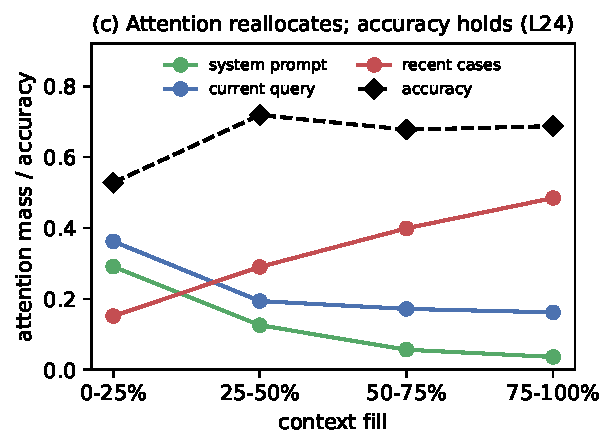
\includegraphics[width=\linewidth]{figures/attention_rot.pdf}\end{subfigure}
  \hfill
  \begin{subfigure}{0.32\textwidth}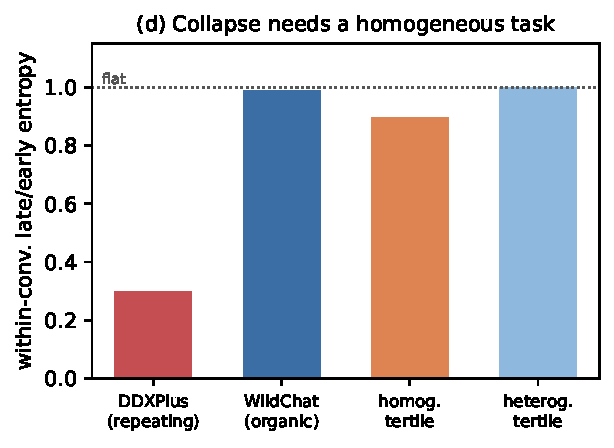
\includegraphics[width=\linewidth]{figures/wildchat_homogeneity.pdf}\end{subfigure}
  \hfill
  \begin{subfigure}{0.32\textwidth}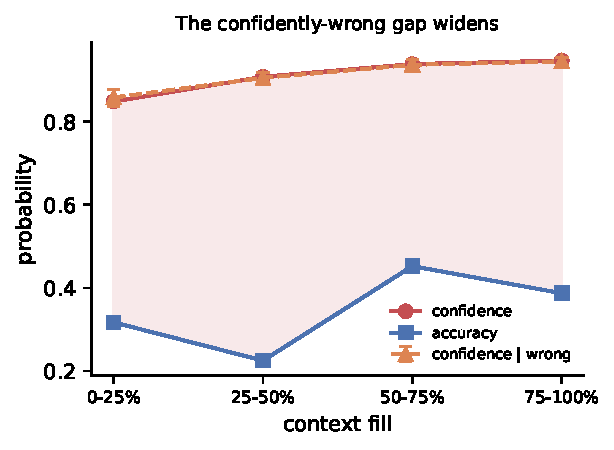
\includegraphics[width=\linewidth]{figures/calibration_gap.pdf}\end{subfigure}
  \caption{\textbf{The signatures are in-context comfort, and the residual hazard is calibration.}
  (a) Attention reallocates monotonically off the system prompt and current query with fill while
  accuracy holds. (b) The entropy collapse appears only with a homogeneous repeating task, not on
  organic WildChat dialogue, and tracks homogeneity rather than length. (c) Confidence rises with
  fill on wrong answers as much as right, at flat accuracy.}
  \label{fig:signatures}
\end{figure}

Consistently, conditioning on fill, the cases OLMo-2 answers \emph{wrong} have \emph{higher}
current-query attention than the ones it gets right (pooled $\Delta=+0.045$ $[-0.003,+0.097]$,
$n{=}115$; sign positive in every fill bin and at every probed layer). Errors are associated with
\emph{fixating} on the query; correct answers spread attention onto the accumulated cases---the
per-case fingerprint of the in-context learning that keeps accuracy up. The ``rot'' and the
within-context predictor of a correct answer point in opposite directions.

\section{Conclusion and Outlook}

\paragraph{Limitations.}
Per-condition $n$ is bounded by the context window, so every interval here depends on the paired
analysis of \S\ref{sec:prelim}; resampling the arms independently inflates each one about $2.5\times$, enough to
report a real effect as null. The necessity direction of the mediation is only partially
established and is plausibly instrument-limited, since the clamp is uniform across heads. The competition result is one
significant step rather than a gradient---mild overlap is indistinguishable from none, and we do
not claim cost rises with confusability. The instruction-canary null is a floor effect, the
WildChat figures are summary values from teacher-forced analyses, and the causal program runs on
one model family. The precedent results are one instruction family, graded by a rule-based
checker at $n{=}40$ per cell; and the carrier of the demonstrated-format mode is unidentified---
it is decodable and installable, but no linear direction we tried erases it, so we localize the
decision neither to a layer nor to a direction. The accuracy null holds for localized tasks; genuinely length-dependent
single-task settings are where dilution is the point, and are out of scope by design.

With accumulation, displacement, competition and precedent separated inside one harness:
accumulation
produces a real, monotone
reallocation of attention and a real collapse of \emph{confidence}, but no loss of accuracy and no
loss of instruction adherence. Displacing the evidence produces a large accuracy cost that is
causally mediated by its attention mass, graded in that mass, and positional in tokens. Making the
context confusable produces a further cost that is \emph{not} mediated by that mass at all.
Accumulating an applicable demonstrated answer shape erodes not accuracy but \emph{compliance},
in a precedent contest the instruction loses with its attention intact---and which either
re-weighting or re-presenting the instruction wins back completely. The literature's central
claim is therefore \emph{correct but misattributed, and under-counted}: context rot is not a
decay with length, it is displacement, competition and precedent, three mechanisms with
different signatures, of which length is merely the usual way of causing them at once.

The residual hazard in the localized case is \emph{calibration}, not competence: on the DDXPlus
streams logging per-token confidence ($n{=}154$ pooled cases, two models, both question orders),
answer confidence rises $0.85\to0.95$ with fill ($r=+0.72$ $[+0.64,+0.79]$) at flat accuracy---and
equally on \emph{wrong} answers ($0.86\to0.95$; $r=+0.69$ $[+0.57,+0.78]$)---so the
confidently-wrong gap widens by ${\sim}10$ points over a session (Fig.~\ref{fig:signatures}c), most
consequential exactly where a homogeneous high-stakes stream makes the model surest. The test we
would run next is the pattern-matched, per-head clamp that would settle whether the partial
necessity above is an instrument limitation or a second channel within displacement itself.

\small
\begin{thebibliography}{9}
\bibitem[Anil et al.(2024)]{anil2024manyshot} C.~Anil et al. Many-shot jailbreaking. \emph{NeurIPS}, 2024.
\bibitem[Camassa and Shiller(2026)]{camassa2026instructioninduction} A.~Camassa and B.~Shiller. Do as I say, not as I do: instruction-induction conflict in LLMs. \emph{arXiv:2605.20382}, 2026.
\bibitem[Cuconasu et al.(2024)]{cuconasu2024noise} F.~Cuconasu et al. The power of noise: redefining retrieval for RAG systems. \emph{SIGIR}, 2024.
\bibitem[Davidson et al.(2025)]{davidson2025taskrepresentation} G.~Davidson, T.~Gureckis, B.~Lake, and A.~Williams. Do different prompting methods yield a common task representation in language models? \emph{NeurIPS}, 2025.
\bibitem[Dongre et al.(2026)]{dongre2026attentioncloses} V.~Dongre et al. When attention closes: how LLMs lose the thread in multi-turn interaction. \emph{arXiv:2605.12922}, 2026.
\bibitem[Hendel et al.(2023)]{hendel2023taskvectors} R.~Hendel, M.~Geva, and A.~Globerson. In-context learning creates task vectors. \emph{Findings of EMNLP}, 2023.
\bibitem[Hendrycks et al.(2021)]{hendrycks2021mmlu} D.~Hendrycks et al. Measuring massive multitask language understanding. \emph{ICLR}, 2021.
\bibitem[Hong et al.(2025)]{hong2025contextrot} K.~Hong, A.~Troynikov, and J.~Huber. Context rot: how increasing input tokens impacts LLM performance. Chroma technical report, 2025.
\bibitem[Laban et al.(2025)]{laban2025lost} P.~Laban, H.~Hayashi, Y.~Zhou, and J.~Neville. LLMs get lost in multi-turn conversation. \emph{arXiv:2505.06120}, 2025.
\bibitem[Levy et al.(2024)]{levy2024same} M.~Levy, A.~Jacoby, and Y.~Goldberg. Same task, more tokens: the impact of input length on the reasoning performance of large language models. \emph{ACL}, 2024.
\bibitem[Liu et al.(2023)]{liu2023lost} N.~F. Liu et al. Lost in the middle: how language models use long contexts. \emph{TACL}, 2023.
\bibitem[Lieberum et al.(2024)]{lieberum2024gemmascope} T.~Lieberum et al. Gemma Scope: open sparse autoencoders everywhere all at once on Gemma 2. 2024.
\bibitem[OLMo Team(2024)]{olmo2024} OLMo Team. OLMo 2: open language models with a full post-training recipe. 2024.
\bibitem[Shi et al.(2023)]{shi2023distracted} F.~Shi et al. Large language models can be easily distracted by irrelevant context. \emph{ICML}, 2023.
\bibitem[Tchango et al.(2022)]{tchango2022ddxplus} A.~Fansi Tchango et al. DDXPlus: a new dataset for automatic medical diagnosis. \emph{NeurIPS Datasets and Benchmarks}, 2022.
\bibitem[Wei et al.(2023)]{wei2023icldifferently} J.~Wei et al. Larger language models do in-context learning differently. \emph{arXiv:2303.03846}, 2023.
\bibitem[Zhao et al.(2024)]{zhao2024wildchat} W.~Zhao et al. WildChat: 1M ChatGPT interaction logs in the wild. \emph{ICLR}, 2024.
\end{thebibliography}

\end{document}
